\setcounter{section}{23}
\setcounter{subsection}{5}
\setcounter{subsubsection}{0}
% Copyright 2019 by Mark Wibrow
%
% This file may be distributed and/or modified
%
% 1. under the LaTeX Project Public License and/or
% 2. under the GNU Free Documentation License.
%
% See the file doc/generic/pgf/licenses/LICENSE for more details.


\section{Decorated Paths\\装饰路径}
\label{section-tikz-decorations}

\subsection{Overview\\概述}

Decorations are a general concept to make (sub)paths ``more interesting''.
Before we have a look at the details, let us have a look at some examples:

装饰是一种使(子)路径“更有趣”的通用概念。在查看详细信息之前,让我们先看一些示例:

%
\begin{codeexample}[preamble={\usetikzlibrary{
    decorations.pathmorphing,
    decorations.pathreplacing,
    decorations.shapes,
}}]
\begin{tikzpicture}[thick]
  \draw                                                (0,3)   -- (3,3);
  \draw[decorate,decoration=zigzag]                    (0,2.5) -- (3,2.5);
  \draw[decorate,decoration=brace]                     (0,2)   -- (3,2);
  \draw[decorate,decoration=triangles]                 (0,1.5) -- (3,1.5);
  \draw[decorate,decoration={coil,segment length=4pt}] (0,1)   -- (3,1);
  \draw[decorate,decoration={coil,aspect=0}]           (0,.5)  -- (3,.5);
  \draw[decorate,decoration={expanding waves,angle=7}] (0,0)   -- (3,0);
\end{tikzpicture}
\end{codeexample}

\begin{codeexample}[preamble={\usetikzlibrary{decorations.pathmorphing}}]
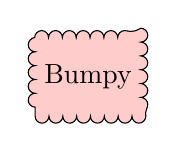
\begin{tikzpicture}
  \node [fill=red!20,draw,decorate,decoration={bumps,mirror},
         minimum height=1cm]
  {Bumpy};
\end{tikzpicture}
\end{codeexample}

\begin{codeexample}[preamble={\usetikzlibrary{decorations.pathmorphing}}]
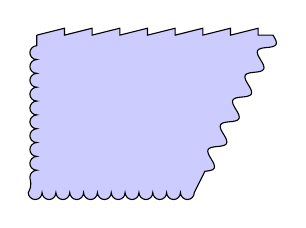
\begin{tikzpicture}
  \filldraw[fill=blue!20]                    (0,3)
  decorate [decoration=saw]             { -- (3,3) }
  decorate [decoration={coil,aspect=0}] { -- (2,1) }
  decorate [decoration=bumps]           { -| (0,3) };
\end{tikzpicture}
\end{codeexample}

\begin{codeexample}[pre={\pgfmathsetseed{1}},preamble={\usetikzlibrary{decorations.pathmorphing}}]
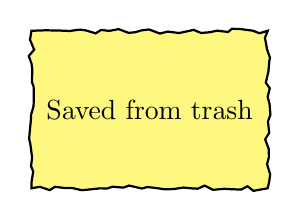
\begin{tikzpicture}
  \node [fill=yellow!50,draw,thick, minimum height=2cm, minimum width=3cm,
         decorate, decoration={random steps,segment length=3pt,amplitude=1pt}]
    {Saved from trash};
\end{tikzpicture}
\end{codeexample}

The general idea of decorations is the following: First, you construct a path
using the usual path construction commands. The resulting path is, in essence,
a series of straight and curved lines. Instead of directly using this path for
filling or drawing, you can then specify that it should form the basis for a
decoration. In this case, depending on which decoration you use, a new path is
constructed ``along'' the path you specified. For instance, with the |zigzag|
decoration, the new path is a zigzagging line that goes along the old path.

装饰的一般思想是:首先,您使用常规的路径构造命令构造一个路径。生成的路径本质上是一系列直线和曲线。您可以指定该路径不直接用于填充或绘制,而是指定它作为装饰的基础。在这种情况下,根据您使用的装饰方式,会在您指定的路径“沿着”上构造一个新的路径。例如,使用 |zigzag| 装饰时,新路径是沿着旧路径的锯齿线。

Let us have a look at an example: In the first picture, we see a path that
consists of a line, an arc, and a line. In the second picture, this path has
been used as the basis of a decoration.

让我们看一个例子:在第一张图片中,我们看到的路径由一条直线、一段弧线和一条直线组成。在第二张图片中,该路径已被用作装饰的基础。

%
\begin{codeexample}[preamble={\usetikzlibrary{decorations.pathmorphing}}]
\tikz \fill
  [fill=blue!20,draw=blue,thick] (0,0) -- (2,1) arc (90:-90:.5) -- cycle;
\end{codeexample}
%
\begin{codeexample}[preamble={\usetikzlibrary{decorations.pathmorphing}}]
\tikz \fill [decorate,decoration={zigzag}]
  [fill=blue!20,draw=blue,thick] (0,0) -- (2,1) arc (90:-90:.5) -- cycle;
\end{codeexample}

It is also possible to decorate only a subpath (the exact syntax will be
explained later in this section).

还可以仅装饰子路径(确切的语法将在本节后面解释)。


\begin{codeexample}[preamble={\usetikzlibrary{decorations.pathmorphing}}]
\tikz \fill [decoration={zigzag}]
  [fill=blue!20,draw=blue,thick] (0,0) -- (2,1)
    decorate { arc (90:-90:.5) } -- cycle;
\end{codeexample}

The |zigzag| decoration will be called a \emph{path morphing} decoration
because it morphs a path into a different, but topologically equivalent path.
Not all decorations are path morphing; rather there are three kinds of
decorations.

|zigzag| 装饰将被称为\emph{路径变形}装饰,因为它将路径变形为不同但拓扑等效的路径。并非所有装饰都是路径变形的;实际上,有三种类型的装饰。

\begin{enumerate}
    \item The just-mentioned \emph{path morphing} decorations morph the path in
        the sense that what used to be a straight line might afterwards be a
        squiggly line or might have bumps. However, a line is still and a line
        and path deforming decorations do not change the number of subpaths.

        刚刚提到的\emph{路径变形}装饰会将路径变形,也就是说,曾经是直线的东西之后可能变成蜿蜒曲折的线条或可能有凹凸。然而,线条仍然是线条,路径变形装饰不会改变子路径的数量。

        Examples of such decorations are the |snake| or the |zigzag|
        decoration. Many such decorations are defined in the library
        |decorations.pathmorphing|.

        这类装饰的示例包括 |snake| 或 |zigzag| 装饰。许多此类装饰在 |decorations.pathmorphing| 库中定义。

        \item \emph{Path replacing} decorations completely replace the path by a
        different path that is only ``loosely based'' on the original path. For
        instance, the |crosses| decoration replaces a path by a path consisting
        of a sequence of crosses. Note how in the following example filling the
        path has no effect since the path consist only of (numerous)
        unconnected straight line subpaths:
        
        \emph{路径替换}装饰会完全用一个完全“基于”原始路径的不同路径替换原始路径。例如,|crosses| 装饰将路径替换为由一系列十字交叉组成的路径。请注意,在下面的示例中,填充路径没有任何效果,因为路径只包含(许多)不相连的直线子路径:


\begin{codeexample}[preamble={\usetikzlibrary{decorations.shapes}}]
\tikz \fill [decorate,decoration={crosses}]
  [fill=blue!20,draw=blue,thick] (0,0) -- (2,1) arc (90:-90:.5) -- cycle;
\end{codeexample}

        Examples of path replacing decorations are |crosses| or |ticks| or
        |shape backgrounds|. Such decorations are defined in the library
        |decorations.pathreplacing|, but also in |decorations.shapes|.

        路径替换装饰的示例包括 |crosses|、|ticks| 或 |shape backgrounds|。此类装饰在 |decorations.pathreplacing| 和 |decorations.shapes| 库中定义。

        \item \emph{Path removing} decorations completely remove the
        to-be-decorated path. Thus, they have no effect on the main path that
        is being constructed. Instead, they typically have numerous \emph{side
        effects}. For instance, they might ``write some text'' along the
        (removed) path or they might place nodes along this path. Note that for
        such decorations the path usage command for the main path have no
        influence on how the decoration looks like.
        
        \emph{路径移除}装饰会完全移除要装饰的路径。因此,它们对正在构建的主路径没有影响。相反,它们通常具有许多\emph{副作用}。例如,它们可能会在(移除的)路径上“写一些文本”,或者可能会在此路径上放置节点。请注意,对于此类装饰,主路径的路径使用命令对装饰的外观没有影响。
\begin{codeexample}[preamble={\usetikzlibrary{decorations.text}}]
\tikz \fill [decorate,decoration={text along path,
               text=This is a text along a path. Note how the path is lost.}]
  [fill=blue!20,draw=blue,thick] (0,0) -- (2,1) arc (90:-90:.5) -- cycle;
\end{codeexample}
        %
\end{enumerate}

Decorations are defined in different decoration libraries, see
Section~\ref{section-library-decorations} for details. It is also possible to
define your own decorations, see Section~\ref{section-base-decorations}, but
you need to use the \pgfname\ basic layer and a bit of theory is involved.

装饰效果在不同的装饰库中定义,详见第~\ref{section-library-decorations}节。您也可以自定义装饰效果,详见第~\ref{section-base-decorations}节,但需要使用\pgfname 的基本层,其中涉及一些理论。

Decorations can be used to decorate already decorated paths. In the following
three graphics, we start with a simple path, then decorate it once, and then
decorate the decorated path once more.

装饰效果可以用于装饰已经装饰过的路径。在下面的三个图形中,我们从一个简单的路径开始,然后装饰它一次,然后再次装饰已经装饰过的路径。

%
\begin{codeexample}[]
\tikz \fill [fill=blue!20,draw=blue,thick]
  (0,0) rectangle (3,2);
\end{codeexample}
%
\begin{codeexample}[preamble={\usetikzlibrary{decorations.pathmorphing}}]
\tikz \fill [fill=blue!20,draw=blue,thick]
  decorate[decoration={zigzag,segment length=10mm,amplitude=2.5mm}]
    { (0,0) rectangle (3,2) };
\end{codeexample}
%
\begin{codeexample}[preamble={\usetikzlibrary{
    decorations.pathmorphing,
    decorations.shapes,
}}]
\tikz \fill [fill=blue!20,draw=blue,thick]
  decorate[decoration={crosses,segment length=2mm}] {
    decorate[decoration={zigzag,segment length=10mm,amplitude=2.5mm}] {
      (0,0) rectangle (3,2)
    }
  };
\end{codeexample}

One final word of warning: Decorations can be pretty slow to typeset and they
can be inaccurate. The reason is that \pgfname\ has to a \emph{lot} of rather
difficult computations in the background and \TeX\ is not very good at doing
math. Decorations are fastest when applied to straight line segments, but even
then they are much slower than other alternatives. For instance, the |ticks|
decoration can be simulated by clever use of a dashing pattern and the dashing
pattern will literally be thousands of times faster to typeset. However, for
most decorations there are no real alternatives.

最后需要提醒的是:装饰效果在排版时可能会非常慢且不准确。原因是\pgfname 在后台进行了很多相当复杂的计算,而\TeX 在进行数学计算时效率不高。当应用于直线段时,装饰效果的速度最快,但即使在这种情况下,它们也比其他替代方案慢得多。例如,可以通过巧妙地使用虚线模式来模拟|ticks|装饰效果,而虚线模式在排版时的速度会比装饰效果快上数千倍。然而,对于大多数装饰效果,实际上没有真正的替代方案。

\begin{tikzlibrary}{decorations}
    In order to use decorations, you first have to load a |decorations| library.
    This |decorations| library defines the basic options described in the
    following, but it does not define any new decorations. This is done by
    libraries like |decorations.text|. Since these more specialized libraries
    include the |decorations| library automatically, you usually do not have to
    bother about it.

    为了使用装饰效果,首先必须加载一个|decorations|库。这个|decorations|库定义了下面描述的基本选项,但它不定义任何新的装饰效果。这是由像|decorations.text|这样的专门库来完成的。由于这些更专业的库会自动包含|decorations|库,所以通常不需要关心它。

  \end{tikzlibrary}


\subsection{Decorating a Subpath Using the Decorate Path Command\\使用装饰路径命令装饰子路径}

The most general way to decorate a (sub)path is the following path command.

装饰(子)路径最通用的方式是使用下面的路径命令。

\begin{pathoperation}{decorate}{\opt{\oarg{options}}\marg{subpath}}
    This path operation causes the \meta{subpath} to be decorated using the
    current decoration. Depending on the decoration, this may or may not extend
    the current path.

    此路径操作使用当前的装饰效果来装饰\meta{subpath}。根据装饰效果,这可能会或可能不会扩展当前路径。

    \begin{codeexample}[preamble={\usetikzlibrary{decorations.pathmorphing}}]
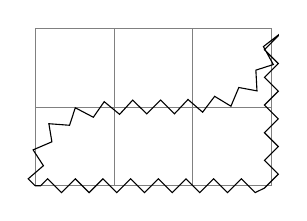
\begin{tikzpicture}
  \draw [help lines] grid (3,2);
  \draw decorate [decoration={name=zigzag}]
         { (0,0) .. controls (0,2) and (3,0) .. (3,2) |- (0,0) };
\end{tikzpicture}
\end{codeexample}
    %
    The path can include straight lines, curves, rectangles, arcs, circles,
    ellipses, and even already decorated paths (that is, you can nest
    applications of the |decorate| path command, see below).

    路径可以包括直线、曲线、矩形、弧线、圆、椭圆,甚至已经装饰过的路径(也就是说,可以嵌套应用|decorate|路径命令,详见下文)。

    Due to the limits on the precision in  \TeX, some inaccuracies in
    positioning when crossing input segment boundaries may occasionally be
    found.

    由于\TeX 的精度限制,在穿越输入线段边界时,可能会偶尔出现一些位置不准确的情况。

    You can use nodes normally inside the \meta{subpath}.

    您可以在\meta{subpath}内正常使用节点。

    %
\begin{codeexample}[preamble={\usetikzlibrary{
    decorations.pathmorphing,
    decorations.shapes,
}}]
\begin{tikzpicture}
  \draw [help lines] grid (3,2);
  \draw decorate [decoration={name=zigzag}]
    { (0,0) -- (2,2) node (hi) [left,draw=red] {Hi!} arc(90:0:1)};

  \draw [blue] decorate [decoration={crosses}] {(3,0) -- (hi)};
\end{tikzpicture}
\end{codeexample}

    The following key is used to select the decoration and also to select
    further ``rendering options'' for the decoration.

    以下关键字用于选择装饰效果,同时还可选择进一步的“渲染选项”:

    \begin{key}{/pgf/decoration=\meta{decoration options}}
            \keyalias{tikz}
        This option is used to specify which decoration is used and how it will
        look like. Note that this key will \emph{not} cause any decorations to
        be applied, immediately. It takes the |decorate| path command or the
        |decorate| option to actually decorate a path. The |decoration| option
        is only used to specify which decoration should be used, in principle.
        You can also use this option at the beginning of a picture or a scope
        to specify the decoration to be used with each invocation of the
        |decorate| path command. Naturally, any local options of the |decorate|
        path command override these ``global'' options.
        %

        此选项用于指定使用的装饰效果及其外观。请注意,此关键字\emph{不会}立即应用任何装饰效果。需要使用|decorate|路径命令或|decorate|选项来实际装饰路径。|decoration|选项仅用于指定应使用的装饰效果,原则上而言。您还可以在图片或作用域的开头使用此选项,以指定在每次调用|decorate|路径命令时要使用的装饰效果。当然,|decorate|路径命令的任何局部选项都会覆盖这些“全局”选项。
        \begin{codeexample}[preamble={\usetikzlibrary{
    decorations.pathmorphing,
    decorations.shapes,
}}]
\begin{tikzpicture}[decoration=zigzag]
  \draw       decorate                      {(0,0) -- (3,2)};
  \draw [red] decorate [decoration=crosses] {(0,2) -- (3,0)};
\end{tikzpicture}
\end{codeexample}

        The \meta{decoration options} are special options (which have the path
        prefix |/pgf/decoration/|) that determine the properties of the
        decoration. Which options are appropriate for a decoration strongly
        depend on the decoration, you will have to look up the appropriate
        options in the documentation of the decoration, see
        Section~\ref{section-library-decorations}.

        \meta{decoration options}是特殊选项(具有路径前缀 |/pgf/decoration/|),用于确定装饰效果的属性。哪些选项适用于装饰效果强烈取决于具体的装饰效果,您需要在装饰效果的文档中查找相应的选项,详见第~\ref{section-library-decorations}节。



        There is one option (available only in \tikzname) that is special:
        
        有一个选项(仅在\tikzname 中可用)是特殊的:

        \begin{key}{/pgf/decoration/name=\meta{name} (initially none)}
            Use this key to set which decoration is to be used. The \meta{name}
            can both be a decoration or a meta-decoration (you need to worry
            about the difference only if you wish to define your own
            decorations).

            使用此关键字设置要使用的装饰效果。 \meta{name} 既可以是装饰效果,也可以是元装饰效果(仅在定义自己的装饰效果时需要区分)。



            If you set \meta{name} to |none|, no decorations are added.
            
            如果将 \meta{name} 设置为 |none|,则不会添加任何装饰效果。

\begin{codeexample}[preamble={\usetikzlibrary{decorations.pathmorphing}}]
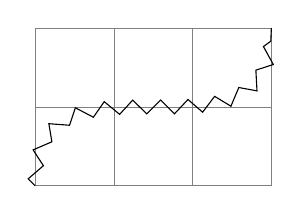
\begin{tikzpicture}
  \draw [help lines] grid (3,2);
  \draw decorate [decoration={name=zigzag}]
         { (0,0) .. controls (0,2) and (3,0) .. (3,2) };
\end{tikzpicture}
\end{codeexample}
            %
            Since this option is used so often, you can also leave out the
            |name=| part. Thus, the above example can be rewritten more
            succinctly:

            由于此选项经常被使用,您也可以省略 |name=| 部分。因此,上面的示例可以更简洁地重写如下:

\begin{codeexample}[preamble={\usetikzlibrary{decorations.pathmorphing}}]
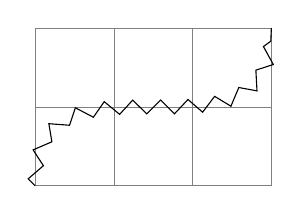
\begin{tikzpicture}
  \draw [help lines] grid (3,2);
  \draw decorate [decoration=zigzag]
         { (0,0) .. controls (0,2) and (3,0) .. (3,2) };
\end{tikzpicture}
\end{codeexample}
            %
            In general, when \meta{decoration options} are parsed, for each
            unknown key it is checked whether that key happens to be a
            (meta-)decoration and, if so, the |name| option is executed for
            this key.

            一般情况下,在解析\meta{decoration options}时,对于每个未知的键,都会检查该键是否恰好是(元)装饰效果,如果是,则为该键执行 |name| 选项。


        \end{key}

        Further options allow you to adjust the position of decorations
        relative to the to-be-decorated path. See
        Section~\ref{section-decorations-adjust} below for details.

        其他选项允许您调整装饰相对于要装饰的路径的位置。有关详细信息,请参见下面的第~\ref{section-decorations-adjust}节。


    \end{key}

    Recall that some decorations actually completely remove the to-be-decorated
    path. In such cases, the construction of the main path is resumed after the
    |decorate| path command ends.
    
    请记住,有些装饰实际上会完全移除要装饰的路径。在这种情况下,在|decorate|路径命令结束后,会恢复主路径的构建。


\begin{codeexample}[preamble={\usetikzlibrary{decorations.text}}]
\begin{tikzpicture}[decoration={text along path,text=
      around and around and around and around we go}]

  \draw (0,0) -- (1,1) decorate { -- (2,1) } -- (3,0);
\end{tikzpicture}
\end{codeexample}

    It is permissible to nest |decorate| commands. In this case, the path
    resulting from the first decoration process is used as the to-be-decorated
    path for the second decoration process. This is especially useful for
    drawing fractals. The |Koch snowflake| decoration replaces a straight line
    like \tikz\draw (0,0) -- (1,0); by
    \tikz[decoration=Koch snowflake] \draw decorate{(0,0) -- (1,0)};.
    Repeatedly applying this transformation to a triangle yields a fractal that
    looks a bit like a snowflake, hence the name.

    允许嵌套|decorate|命令。在这种情况下,第一个装饰过程生成的路径被用作第二个装饰过程的要装饰路径。这对于绘制分形特别有用。|Koch snowflake|装饰将一条直线,比如\tikz\draw (0,0) -- (1,0);,替换为\tikz[decoration=Koch snowflake] \draw decorate{(0,0) -- (1,0)};。将此转换反复应用于一个三角形将产生一个类似雪花的分形,因此得名。


    %
\begin{codeexample}[preamble={\usetikzlibrary{decorations.fractals}}]
\begin{tikzpicture}[decoration=Koch snowflake,draw=blue,fill=blue!20,thick]
  \filldraw (0,0) -- ++(60:1) -- ++(-60:1) -- cycle ;
  \filldraw decorate{ (0,-1) -- ++(60:1) -- ++(-60:1) -- cycle };
  \filldraw decorate{ decorate{ (0,-2.5) -- ++(60:1) -- ++(-60:1) -- cycle }};
\end{tikzpicture}
\end{codeexample}
    %
\end{pathoperation}


\subsection{Decorating a Complete Path\\装饰完整路径}

You may sometimes wish to decorate a path over whose construction you have no
control. For instance, the path of the background of a node is created without
having a chance to issue a |decorate| path command. In such cases you can use
the following option, which allows you to decorate a path ``after the fact''.

有时您可能希望装饰一个您无法控制其构造的路径。例如,节点的背景路径是在没有机会发出|decorate|路径命令的情况下创建的。在这种情况下,您可以使用以下选项,在“事后”装饰路径。



\begin{key}{/tikz/decorate=\opt{\meta{boolean}} (default true)}
    When this key is set, the whole path is decorated after it has been
    finished. The decoration used for decorating the path is set via the
    |decoration| way, in exactly the same way as for the |decorate| path
    command. Indeed, the following two commands have the same effect:
    
    设置此键后,整个路径在完成后进行装饰。用于装饰路径的装饰方式通过|decoration|方式设置,与|decorate|路径命令完全相同。实际上,以下两个命令具有相同的效果:


    \begin{enumerate}
        \item |\path decorate[|\meta{options}|] {|\meta{path}|};|
        \item |\path [decorate,|\meta{options}|] |\meta{path}|;|
    \end{enumerate}
    %
    The main use or the |decorate| option is the you can also use it with the
    nodes. It then causes the background path of the node to be decorated. Note
    that you can decorate a background path only once in this manner. That is,
    in contrast to the |decorate| path command you cannot apply this option
    twice (this would just set it to |true|, once more).
    
    |decorate|选项的主要用途是可以与节点一起使用。它会导致节点的背景路径被装饰。请注意,只能以此方式装饰背景路径一次。也就是说,与|decorate|路径命令不同,您不能两次应用此选项(这只会将其设置为|true|,再多一次)。


\begin{codeexample}[preamble={\usetikzlibrary{
    decorations.pathmorphing,
    decorations.text,
    shapes.geometric,
}}]
\begin{tikzpicture}[decoration=zigzag]
  \draw [help lines] (0,0) grid (3,5);

  \draw [fill=blue!20,decorate] (1.5,4) circle (1cm);

  \node at (1.5,2.5) [fill=red!20,decorate,ellipse] {Ellipse};

  \node at (1.5,1) [inner sep=6mm,fill=red!20,decorate,ellipse,decoration=
    {text along path,text={This is getting silly}}] {Ellipse};
\end{tikzpicture}
\end{codeexample}

    In the last example, the |text along path| decoration removes the path. In
    such cases it is useful to use a pre- or postaction to cause the decoration
    to be applied only before or after the main path has been used.
    Incidentally, this is another application of the |decorate| option that you
    cannot achieve with the decorate path command.
    
    在最后一个示例中,|text along path|装饰移除了路径。在这种情况下,使用预操作或后操作将装饰应用于主路径之前或之后非常有用。顺便说一句,这是|decorate|选项的另一个应用,您无法使用装饰路径命令实现此效果。


\begin{codeexample}[preamble={\usetikzlibrary{
    decorations.pathmorphing,
    decorations.text,
    shapes.geometric,
}}]
\begin{tikzpicture}[decoration=zigzag]
  \node at (1.5,1) [inner sep=6mm,fill=red!20,ellipse,
    postaction={decorate,decoration=
    {text along path,text={This is getting silly}}}] {Ellipse};
\end{tikzpicture}
\end{codeexample}
    %
    Here is more useful example, where a postaction is used to add the path
    after the main path has been drawn.
    
    这里有一个更有用的示例,其中使用后操作在绘制主路径之后添加路径。


% \catcode`\|12 % !?
\begin{codeexample}[preamble={\usetikzlibrary{decorations.text}}]
\begin{tikzpicture}
\draw [help lines] grid (3,2);
\fill [draw=red,fill=red!20,
         postaction={decorate,decoration={raise=2pt,text along path,
           text=around and around and around and around we go}}]
  (0,1) arc (180:-180:1.5cm and 1cm);
\end{tikzpicture}
\end{codeexample}
    %
\end{key}


\subsection{Adjusting Decorations\\调整装饰}
\label{section-decorations-adjust}

\subsubsection{Positioning Decorations Relative to the To-Be-Decorate Path\\将装饰相对于待装饰路径进行定位}

The following option, which are only available with \tikzname, allow you to
modify the positioning of decorations relative to the to-be-decorated path.

以下选项仅适用于\tikzname,允许您修改装饰相对于待装饰路径的定位。

\begin{key}{/pgf/decoration/raise=\meta{dimension} (initially 0pt)}
    The segments of the decoration are raised by \meta{dimension} relative to
    the to-be-decorated path. More precisely, the segments of the path are
    offset by this much ``to the left'' of the path as we travel along the
    path. This raising is done after and in addition to any transformations set
    using the |transform| option (see below).

    装饰的片段相对于待装饰路径提升了\meta{dimension}。更准确地说,当我们沿着路径行进时,路径的片段沿着路径的“左侧”偏移这么多。这种提升是在使用|transform|选项设置的任何变换之后和之外进行的(参见下文)。

    A negative \meta{dimension} will offset the decoration ``to the right'' of
    the to-be-decorated path.

    负的\meta{dimension}将装饰物沿着待装饰路径“右侧”偏移。
    %
\begin{codeexample}[preamble={\usetikzlibrary{decorations.shapes}}]
\begin{tikzpicture}
  \draw [help lines] (0,0) grid (3,2);

  \draw (0,0) -- (1,1) arc (90:0:2 and 1);
  \draw      decorate [decoration=crosses]
        { (0,0) -- (1,1) arc (90:0:2 and 1) };
  \draw[red] decorate [decoration={crosses,raise=5pt}]
        { (0,0) -- (1,1) arc (90:0:2 and 1) };
\end{tikzpicture}
\end{codeexample}
    %
\end{key}

\begin{key}{/pgf/decoration/mirror=\opt{\meta{boolean}}}
    Causes the segments of the decoration to be mirrored along the
    to-be-decorated path. This is done after and in addition to any
    transformations set using the |transform| and/or |raise| options.
    
    使装饰的片段沿着待装饰路径镜像。这是在使用|transform|和/或|raise|选项设置的任何变换之后和之外进行的。


\begin{codeexample}[preamble={\usetikzlibrary{decorations.pathreplacing}}]
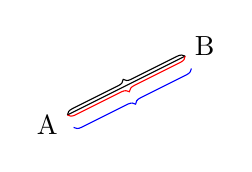
\begin{tikzpicture}
  \node (a)          {A};
  \node (b) at (2,1) {B};
  \draw                                                    (a) -- (b);
  \draw[decorate,decoration=brace]                         (a) -- (b);
  \draw[decorate,decoration={brace,mirror},red]            (a) -- (b);
  \draw[decorate,decoration={brace,mirror,raise=5pt},blue] (a) -- (b);
\end{tikzpicture}
\end{codeexample}
    %
\end{key}

\begin{key}{/pgf/decoration/transform=\meta{transformations}}
    This key allows you to specify general \meta{transformations} to be applied
    to the segments of a decoration. These transformations are applied before
    and independently of |raise| and |mirror| transformations. The
    \meta{transformations} should be normal \tikzname\ transformations like
    |shift| or |rotate|.

    此键允许您指定应应用于装饰片段的一般\meta{transformations}。这些变换在|raise|和|mirror|变换之前和之外应用。\meta{transformations}应该是正常的\tikzname 变换,如|shift|或|rotate|。

    In the following example the |shift only| transformation is used to make
    sure that the crosses are \emph{not} sloped along the path.

    在下面的示例中,使用|shift only|变换确保十字架\emph{不}沿着路径倾斜。
    %
\begin{codeexample}[preamble={\usetikzlibrary{decorations.shapes}}]
\begin{tikzpicture}
  \draw [help lines] (0,0) grid (3,2);

  \draw (0,0) -- (1,1) arc (90:0:2 and 1);
  \draw[red,very thick] decorate [decoration={
               crosses,transform={shift only},shape size=1.5mm}]
        { (0,0) -- (1,1) arc (90:0:2 and 1) };
\end{tikzpicture}
\end{codeexample}
    %
\end{key}


\subsubsection{Starting and Ending Decorations Early or Late\\提前或推迟开始和结束装饰}

You sometimes may wish to ``end'' a decoration a bit early on the path. For
instance, you might wish a |snake| decoration to stop 5mm before the end of the
path and to continue in a straight line. There are different ways of achieving
this effect, but the easiest may be the |pre| and |post| options, which only
have an effect in \tikzname. Note, however, that they can only be used with
decorations, not with meta-decorations.

有时您可能希望在路径上稍早“结束”装饰。例如,您可能希望|snake|装饰在路径末端前5mm停止,并在直线上继续。有不同的方法可以实现这种效果,但最简单的方法可能是使用|pre|和|post|选项,它们只对\tikzname 有效。但请注意,它们只能用于装饰,而不能用于元装饰。

\begin{key}{/pgf/decoration/pre=\meta{decoration} (initially lineto)}
    This key sets a decoration that should be used before the main decoration
    starts. The \meta{decoration} will be used for a length of |pre length|,
    which |0pt| by default. Thus, for the |pre| option to have any effect, you
    also need to set the |pre length| option.

    此键设置了一个在主装饰开始之前应使用的装饰。默认情况下,\meta{decoration} 将用于 |pre length| 的长度,该长度默认为 |0pt|。因此,为了使 |pre| 选项产生任何效果,您还需要设置 |pre length| 选项。


    %
    % TODO: Nesting tikzpictures is NOT supported 
\begin{codeexample}[preamble={\usetikzlibrary{decorations.pathmorphing}}]
\tikz [decoration={zigzag,pre=lineto,pre length=1cm}]
  \draw [decorate] (0,0) -- (2,1) arc (90:0:1);
\end{codeexample}
    %
\begin{codeexample}[preamble={\usetikzlibrary{decorations.pathmorphing}}]
\tikz [decoration={zigzag,pre=moveto,pre length=1cm}]
  \draw [decorate] (0,0) -- (2,1) arc (90:0:1);
\end{codeexample}
    %
\begin{codeexample}[preamble={\usetikzlibrary{
    decorations.pathmorphing,
    decorations.shapes,
}}]
\tikz [decoration={zigzag,pre=crosses,pre length=1cm}]
  \draw [decorate] (0,0) -- (2,1) arc (90:0:1);
\end{codeexample}

    Note that the default |pre| option is |lineto|, not |curveto|. This means
    that the default |pre| decoration will not follow curves (for efficiency
    reasons). Change the |pre| key to |curveto| if you have a curved path.
    
    注意,默认的 |pre| 选项是 |lineto|,而不是 |curveto|。这意味着默认的 |pre| 装饰不会沿曲线绘制(出于效率原因)。如果您有一条曲线路径,请将 |pre| 键更改为 |curveto|。


\begin{codeexample}[preamble={\usetikzlibrary{decorations.pathmorphing}}]
\tikz [decoration={zigzag,pre length=3cm}]
  \draw [decorate] (0,0) -- (2,1) arc (90:0:1);
\end{codeexample}
    %
\begin{codeexample}[preamble={\usetikzlibrary{decorations.pathmorphing}}]
\tikz [decoration={zigzag,pre=curveto,pre length=3cm}]
  \draw [decorate] (0,0) -- (2,1) arc (90:0:1);
\end{codeexample}
    %
\end{key}

\begin{key}{/pgf/decoration/pre length=\meta{dimension} (initially 0pt)}
    This key sets the distance along which the pre-decoration should be used.
    If you do not need/wish a pre-decoration, set this key to |0pt| (exactly
    this string, not just to something that evaluates to the same things such
    as |0cm|).

    此键设置了应使用预装饰的距离。如果您不需要或不希望预装饰,请将此键设置为 |0pt|(确切地说,不仅仅是评估为相同内容的内容,例如 |0cm|)。


\end{key}

\begin{key}{/pgf/decorations/post=\meta{decoration} (initially lineto)}
    Works like |pre|, only for the end of the decoration.

    与 |pre| 类似,只不过用于装饰的末尾。

\end{key}

\begin{key}{/pgf/decorations/post length=\meta{dimension} (initially 0pt)}
    Works like |pre length|, only for the end of the decoration.

    与 |pre length| 类似,只不过用于装饰的末尾。
\end{key}

Here is a typical example that shows how these keys can be used:

下面是一个典型的示例,展示了如何使用这些键:

\begin{codeexample}[preamble={\usetikzlibrary{decorations.pathmorphing}}]
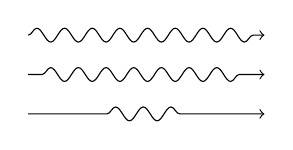
\begin{tikzpicture}
  [decoration=snake,
   line around/.style={decoration={pre length=#1,post length=#1}}]

  \draw[->,decorate]                  (0,0)    -- ++(3,0);
  \draw[->,decorate,line around=5pt]  (0,-5mm) -- ++(3,0);
  \draw[->,decorate,line around=1cm]  (0,-1cm) -- ++(3,0);
\end{tikzpicture}
\end{codeexample}
